%option->configure texmaker->edit-> lato medium 16
\documentclass[12pt]{article}
\usepackage{amsmath}

\usepackage{indentfirst}
\usepackage[font=scriptsize]{caption}
%\usepackage[font=small]{caption}10
%\usepackage[font=footnotesize]{caption}%9
%\usepackage[font=scriptsize]{caption}%8

\usepackage[utf8]{inputenc}
\usepackage{graphicx}
\usepackage{hyperref}
\usepackage[letterpaper,margin=0.5in]{geometry}
\usepackage{setspace}
\usepackage{comment}
\usepackage{amsmath}
\usepackage{esint}
\usepackage{wrapfig}
\usepackage{lipsum}
\usepackage{subcaption}
\usepackage{caption}

\begin{document}

\doublespacing

\begin{center}
{\Large \textbf{Developments of a Simple Model to Elucidate the Shape of Enveloped Viruses: Motivated by Monkeypox and SARS-CoV-2}}\\[1.5ex]
{\normalsize  Hua Deng}\\

{\normalsize February 21, 2025}
\end{center}


\begin{flushleft}
\setlength{\parindent}{30pt}
\section*{Specific aim}


First, our goal is to develop models and simulations combining polymer and liquid-state physics to study how viral genome properties—shape, length, and flexibility—influence membrane morphology. By simulating genome behavior in confined spaces, we intend to uncover key principles of viral assembly and stability, informing strategies to prevent and treat infections like Monkeypox and SARS-CoV-2.

Second, understanding internal pressure in viruses uncovers how they inject their genomes into host cells. Packaging builds up pressure that drives rapid genome release. Studying this process may lead to antiviral strategies targeting genome packaging, inspire virus-like drug delivery systems, improve vaccine design, and deepen our understanding of nucleic acids under extreme confinement.
\vspace{-1em} 
\section*{Motivation}

Previously, we investigated how spherical monomers self-organize into dimers, trimers, and tetramers on spherical surfaces, inspired by the trimeric spike proteins found in COVID-19 viruses. Using Monte Carlo simulations with an anistropic attraction and excluded volume repulsion between monomers, we identified the conditions that trimer formation becomes a favorable process. Both interaction energy form and interaction strength are crucial to surpass the entropically favorable dimers.  By adjusting the angular part of the anistropic interaction, tetramers become the major specie. The simulated trimers are consistent with structural observations from cryo-electron microscopy studies of SARS-CoV-2 spike proteins\cite{Ke2020}. 


Building on the foundation of our previous studies, we intend to develop a simple coarse-grained model with minimal parameters to elucidate how the interplay between the membrane and the enclosed genome regulates the shape of enveloped viruses. The goal of this approach is to provide deeper thermodynamic insights into viral interior organization above molecular length scales, the mutual influence between the membrane and genome, and the internal pressure created by viral genetic materials —knowledge that could inform the development of new antiviral strategies.

\begin{figure}[!ht]
  \centering
  \includegraphics[width=0.8\textwidth,height=4cm]{spike.trimer.png}
  \caption{Left image: Simulation of the SARS-CoV-2 spike protein on a spherical surface, illustrating the progression from randomly distributed monomers (left) to trimer (center) and tetramer (right) formations. Right image: SARS-CoV-2 for Covid-19 schematic image ( CDC Public
Health Image Library) \cite{cdc-covid}}
\end{figure}

%\vspace{-1em} 
\section*{Background and Significance}


Viral infections significantly impact global health, driving pandemics and outbreaks. Enveloped viruses like Monkeypox and COVID-19 are surrounded by lipid membranes that protect their genomes and enable infection by interacting with host cell receptors. Understanding these mechanisms is key to developing effective treatments.

Virions are acellular particles lacking cellular structures such as organelles or membranes.
The shape of enveloped viruses is influenced by their genomes. Monkeypox virus has a $\sim190$ kb 

\begin{figure}[!ht]
  \centering  
  \fbox{\includegraphics[width=0.4\textwidth,height=4cm]{electron.monkeypox.png}}
  \caption{Electron microscopic (EM) image for
Monkeypox virus particles. Oval-shaped
virus particles are mature, and spherical
particles are immature virions \cite{goldsmith2003monkeypox}}
\end{figure}

\noindent double-stranded DNA genome ($\sim3000$ nm contour length), much larger than the $\sim250$ nm virus particle \cite{erez2019diagnosis}\cite{parker2007human}. As shown in Figure 2, immature viruses are spherical, while mature forms appear oval.


This study investigates how genome shape influences membrane morphology in virus particles, focusing on the transition from spherical (immature) to oval (mature) forms. Using a coarse-grained model and Monte Carlo simulations, we will examine how genome compaction, fluctuations, and spatial arrangement drive membrane deformation during virus maturation.









In contrast, SARS-CoV-2 particles are smaller (~80–120 nm) and spherical, with a single $\sim30$ kb RNA genome ($\sim1,400$ nm contour length) \cite{baron2020sars}\cite{Wu2022}. SARS-CoV-2 infects host cells by binding its spike (S) protein to the ACE2 receptor, facilitating entry through membrane fusion or endocytosis \cite{Barrow2013}\cite{payne2022viruses}.

\begin{figure}[htbp]
  \centering
  \begin{subfigure}[t]{0.45\textwidth}
    \centering
    \vtop{\null
      \hbox{\fbox{\includegraphics[width=\linewidth,height=4.5cm]{endocytosis.png}}}
      \caption{Illustration of the steps of virus entry via clathrin-mediated endocytosis. (A) Virus approaches the cell surface. (B) Biochemical interactions between ligands and receptors attract virus to the cell surface. (C) Virus attaches to the cell surface and signals the cell. (D) A clathrin-coated pit is formed around the bound virus. (E) A clathrin-coated vesicle is formed, and the dynamin at the neck region facilitates vesicle scission. (F) The vesicle travels to the cell interior \cite{Barrow2013}.}
      \label{fig:endocytosis}
    }
  \end{subfigure}
  \hfill
  \begin{subfigure}[t]{0.45\textwidth}
    \centering
    \vtop{\null
      \hbox{\fbox{\includegraphics[width=\linewidth,height=4.5cm]{fusion.png}}}
      \caption{Membrane fusion. Many viruses, both enveloped and unenveloped, are brought into cells by endocytosis. The low pH environment in the endosome triggers molecular rearrangements of capsid or envelope proteins. In this example, an enveloped virus is fusing with an endosomal membrane to release the capsid into the cytosol \cite{payne2022viruses}.}
      \label{fig:fusion}
    }
  \end{subfigure}

  \caption{Comparison of virus entry mechanisms: (a) Clathrin-mediated endocytosis, and (b) Membrane fusion.}
  \label{fig:sidebyside}
\end{figure}



After entering the host cell, the viral envelope is removed, releasing its  RNA genome into the cytoplasm. This RNA acts as mRNA, directing the host’s ribosomes to produce viral proteins, including spike proteins, structural proteins, and enzymes for replication. The genome is also copied to make new RNA strands. These components assemble into new viruses, which exit the cell by budding, acquiring a portion of the host membrane with spike proteins. 
 
Unlike Monkeypox virus, which changes from spherical to oval shapes, SARS-CoV-2 stays spherical throughout its life cycle. This study uses coarse-grained models and Monte Carlo simulations, adjusting genome length and membrane size to SARS-CoV-2 dimensions, to investigate how genome compaction and arrangement affect membrane deformation. The goal is to reveal general physical constraints on genome–membrane interactions influencing viral assembly and stability across viruses from thermodynamic standpoints.
%------------------------------------------------------------------------------------------------------------------

A key question is how viruses generate and release internal pressure to inject their genomes into host cells. During assembly, ATP-powered motors tightly pack DNA or RNA into capsids or membranes, creating high pressure—often tens of atmospheres. This pressure arises from electrostatic repulsion between negatively charged nucleic acids and bending strain from compressing a long, rigid molecule into a confined space\cite{BrandarizNunez2019}. Viral pressurization drives rapid genome ejection for fast infection. Using coarse-grained models and Monte Carlo simulations, we will study how genome packing and membrane or capsid deformation generate these forces. This may identify antiviral targets to block pressure-driven ejection and prevent infection.

%\vspace{-5em} 
\section*{Research Plan}
%\vspace{-1em}
\subsection*{I. Techniques}
%\vspace{-1em}
 \subsection*{\indent{1. Coarse-Grained Models (CGM)}}





\begin{figure}[!ht]
  \centering
  \fbox{\includegraphics[width=0.55\textwidth,height=4cm]{discrete.png} }
  \caption{Different computational methods developed to study cellular membranes are valid in different length and time scales.\cite{chabanon2017systems}}
\end{figure}

It simplifies complex systems by grouping atoms or molecules into larger particles called beads. This enables large-scale simulations with reduced computational cost and identifying minimal-parameter models.



\vspace{-1em}
\subsection* {\indent {2. Continuum models}}


Besides treating solvents as dielectric continuum, the continuum model excludes molecular details like lipid composition, phase transitions, and specific atomistic interactions, and cannot capture small atomic-scale fluctuations. However, it efficiently studies large-scale membrane shapes and mechanics, capturing bending and tension without high computational cost. (Note that phase transitions have been argued as a possible driving force to induce cellular self-organization.)



\subsection*{\indent{3. Monte Carlo Simulation (MC)}}





Metropolis rule:
\begin{equation}
P = \min\left(1, e^{-\beta \Delta E}\right)
\end{equation}

This is a key expression in the Metropolis-Hastings algorithm, often used in Monte Carlo simulations, to determine the acceptance probability of a proposed move in a system. $P$: Probability of accepting the proposed move; if accepted, positions update, otherwise the move is reverted.
$\Delta E$: Energy change from the move ($E_{\text{new}} - E_{\text{old}}$).
$\beta$: Inverse temperature factor, $\beta = 1 / (k_B T)$, from the Boltzmann distribution. 
If $\Delta E \leq 0$, the move is always accepted ($P = 1$) since it leads to a lower-energy, more favorable state.
 

\subsection*{II. Procedure and Methods} 


These are the specific models and procedures implemented using the above techniques.\\

 

  \subsection*{\indent{1. Helfrich–Canham Membrane Model}}

  	 \indent\indent(1)Describes membrane bending energy:

\vspace{-1em}
\begin{align}
F_\text{full mem} = \int_S \Bigg[
&\underbrace{\frac{\kappa}{2} \left(2H - C_0(\vec{r}) \right)^2}_{(1)\ \text{spontaneous-curvature-modified bending}} 
\ + \ 
\underbrace{\bar{\kappa} K}_{(2)\ \text{Gaussian-curvature term}} 
\Bigg] dA \nonumber \\
&\quad + \ 
\underbrace{\lambda A}_{(3)\ \text{area constraint}} 
\ + \ 
\underbrace{p V}_{(4)\ \text{volume constraint}}.
\end{align}

\indent\indent (2)Discrete angle-based version used for simulations.

\begin{equation}
E_{\text{bend}} = \kappa \sum_{\langle i,j \rangle} \left(1 - \cos \theta_{ij} \right)+\lambda A+p V
\end{equation}

 \subsection*{\indent{ 2. Kremer–Grest Bead-Spring Model for genome}}

       

       \indent \indent (1) FENE potential for bonded interactions. Finitely Extensible Nonlinear 
Elastic spring 
\indent \indent keeps beads connected but prevents them from stretching too far 
 or breaking

\begin{equation}
U_{\text{FENE}}(r) = -\frac{1}{2} k R_0^2 \ln \left[ 1 - \left( \frac{r}{R_0} \right)^2 \right]
\end{equation}


          \indent\indent   (2) WCA potential, a purely repulsive form of the Lennard-Jones (LJ) potential 
          \indent \indent for excluded volume (non-bonded interactions).
          
\begin{equation}
U_{\text{WCA}}(r) = 
\begin{cases}
4\varepsilon \left[ \left( \dfrac{\sigma}{r} \right)^{12} - \left( \dfrac{\sigma}{r} \right)^6 \right] + \varepsilon, & \text{if } r \leq 2^{1/6} \sigma \\
0, & \text{if } r > 2^{1/6} \sigma
\end{cases}
\end{equation}
\begin{comment}
\subsection*{\indent{3. Monte Carlo Move Set}}

    \indent\indent(1)Randomly displace particles (DNA beads, crowders, or membrane vertices).

   \indent\indent(2) Accept/reject moves using: Metropolis criterion
\end{comment}

\begin{comment}
%\setlength{\parindent}{0pt}
\begin{equation}
P_{\text{accept}} = \min \left(1, e^{-\beta \Delta E}\right)
\end{equation}
\end{comment}
    


\subsection*{\indent{3. Simple Liquid Models}}

       
Simple liquid models that help understand the structure and behavior of polymer in crowded environments. Specifically, the simple liquid models referenced include Hard Sphere Model and Lennard-Jones Model. 

Hard sphere model is used to understand the behavior of particles in crowded environments, where the excluded volume effect becomes important. 

The Lennard-Jones model accounts for both attractive and repulsive forces between particles, which is important in understanding the interactions within fluids and condensed matter. It helps model the behavior of molecules, especially in non-ideal conditions like those found in crowded environments.
\begin{equation}
E = E_{\text{mem-bend}}+\sum_{\text{DNA-bonds}} U_{\mathrm{FENE}} + \sum_{\text{DNA-nonbonded}} U_{\mathrm{WCA}} 
+ \sum_{\text{DNA-crowder}} U_{\mathrm{LJ}} 
+ \sum_{\text{crowder-crowder}} U_{\mathrm{LJ}}
\end{equation} 

  \subsection*{\indent{4. Excluded Volume Implementation}}
Excluded volume is essential in coarse-grained modeling to prevent particle overlap and ensure physical realism. This is enforced using repulsive potentials, such as the Lennard-Jones potential, with carefully chosen bead size ($\sigma$) and interaction strength ($\varepsilon$). Energy minimization and equilibration are performed before simulations to remove overlaps and stabilize the system. Proper excluded volume enforcement is critical for maintaining structural integrity and accurate thermodynamics in biomolecular and polymer simulations.

\subsection*{\indent{5. Ensemble Settings}}

(1) NVT (Canonical Ensemble): 

In an NVT simulation, the number of beads, the volume, and the temperature are kept constant throughout the simulation.  As the simulation progresses, the beads move and interact according to physical forces, leading to fluctuations in pressure and energy, even though the temperature remains stable. 
\begin{equation}
P_{\text{accept}} = \min \left( 1, \exp\left[-\frac{\Delta E}{k_B T}\right] \right)
\end{equation}

In an NVT simulation, pressure fluctuates as beads move and interact. Plotting pressure versus Monte Carlo steps shows these changes. Total energy also fluctuates but remains near an average value. Plotting total energy over time helps check if the system is equilibrated.
   
   

(2) NPT (Isothermal–Isobaric Ensemble): 

In an NPT simulation, the number of particles, pressure, and temperature are constant, while the volume fluctuates. As beads interact, the membrane can expand or contract to balance pressure, causing changes in density and structure. Bead positions, velocities, energy, and membrane size continuously evolve.
        
\begin{equation}
P_{\text{accept}} = \min \left( 1, \exp \left[ - \frac{\Delta E + p \Delta V - N k_B T \ln \left( \frac{V_{\text{new}}}{V_{\text{old}}} \right)}{k_B T} \right] \right)
\end{equation}
 
After obtaining simulation data, volume fluctuations at fixed pressures and temperatures will be analyzed. Average volume will be calculated and plotted against pressure. Additionally, volume and energy fluctuations over time will be examined to assess stability and equilibration, providing insight into the membrane’s pressure response. 

\subsection*{\indent{6. Pressure Calculation by Theoretical Model}}

Previous studies, such as Grayson et al.\cite{Grayson2006}, modeled DNA packaging energy by representing the capsid as a sphere and the genome as an extended semiflexible rod. Similarly, we model the membrane as a spherical enclosure and the RNA as an extended semiflexible rod.

Our goal is to quantify how the structure of the genome influences the internal pressure within the membrane. Specifically, we aim to understand how changes in the RNA persistence length  \(\xi\)\ and the radial loop distribution \(N(r)\) affect the pressure \(P\).  To estimate it, we divide the total bending energy of the RNA by the volume of the membrane.  






\begin{equation}
P = \frac{\sqrt{3} k_B T \, \xi^2}{R^3} \int_{R_\text{in}}^{R_\text{out}} \frac{N(r)}{r} \, dr
\end{equation}

\begin{comment}
\subsection*{Simulation Procedures}
(1)Initialization of DNA chains and crowders.

(2) Energy calculation (FENE + WCA/LJ).

(3) Repeated Monte Carlo updates to reach equilibrium.
\end{comment}



\subsection*{\indent{7. Pressure Calculation by Primitive Model}}
We use the Primitive Model (PM) to simulate the pressure exerted by the genome as it passes through a narrow slit in the membrane. Primitive Model (PM)	is a specific type of coarse-grained model that uses minimal physics (e.g., hard spheres + short-range bonding) to capture essential behavior.

 
In our research, the genome chain, represented as a series of beads connected by covalent bonds, translocates through a small slit in the membrane, and each bead is treated as a rigid, impenetrable sphere with a diameter $ \sigma $. The contact theorem\cite{Voertler1997} applies by relating the pressure normal to the slit walls, $ p_w $, to the one-particle density of these beads at the contact distance $ z = \sigma/2 $, expressed as 


\begin{equation}
{p_w}= \rho(z) *kT \quad \text{for} \quad z \to \frac{L - \sigma}{2}
\end{equation}


\begin{comment}
\subsection*{Simulation Procedures}

(1)Genome modeled as hard spheres (Primitive Model).

(2)Confined in a slit geometry.

(3)Simulate genome movement and collisions.

(4)Measure bead density at wall contact.

(5)Compute pressure using contact theorem
\end{comment}


\subsection*{III. Hypothesis}
\begin{comment}
\noindent \textbf{Hypothesis 1:}\\
The shape of a virus forms after its genome architecture stabilizes. First, the genome reaches a steady state, and we then examine how it influences the viral membrane shape. 

\noindent \textbf{Hypothesis 2:}\\
The genome architecture may develop after the viral membrane shape stabilizes. In this case, the membrane reaches a steady state first, and we then observe how it affects the genome’s geometry. By adjusting the length of 1D rod or the perimeter of the circle of the genome, we try to match the reference.\cite{goldsmith2003monkeypox}\\

\noindent \textbf{Hypothesis 3}:\\
The shape of a virus and its genome architecture form simultaneously.
The model for this hypothesis allows both genome morphology and membrane shape to undergo simultaneous
fluctuation until both arrive at a mutual steady state.
\end{comment}

\noindent \textbf{Hypothesis 1}:\\
Virus shape and genome structure develop through interactions where either the genome or membrane stabilizes first, or both stabilize together. Changing genome length or shape lets the model reproduce these behaviors and match experiments.
	
\noindent \textbf{Hypothesis 2:}\\
In simulations of genome translocation through a narrow membrane slit, the pressure normal to the slit walls calculated using the contact theorem in the Primitive Model—based on the bead density at the slit surface—will agree with the pressure predicted by the Theoretical Model.

\subsection*{IV.Expected outcomes} 
%\subsection*{IV.Possible pitfalls} 
(1)The shape of a virus and its genome architecture form simultaneously.
	
\begin{figure}[!ht]
  \centering
  \fbox{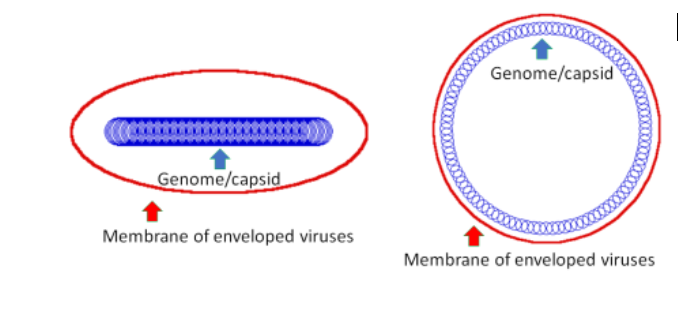
\includegraphics[width=0.5\textwidth,height=3.7cm]{monkeypox.png}}  % Adjust width or height as needed
  \caption{Preliminary 2D model studies to
investigate the effect of the geometry of a
genome on the shape of a virus. A rod-like
genome induces an elliptic shape whereas a
circular genome leads to a circular shape\cite{goldsmith2003monkeypox}.}
\end{figure}

(2)The expectation that different methods for calculating the pressure in a Monte Carlo simulation of a system, such as the primitive model (PM) of genome in slit-like pores should yield consistent values for the pressure normal to the walls of membrane, assuming the methods are correctly implemented and the system is properly equilibrated.

\subsection*{V.Projected timeline}

Months 0-3: Fine-tune the continuum membrane model.\\
Months 4-6: Investigate competition among different membrane shapes.\\
Months 7-9: Study chain model and crowding effect\\
Months 10-12:Expand the developed models from 2D to 3D.\\


\newpage

\subsection*{Extra source}
Rod Bent Into a Circle:
\begin{equation}
E = \frac{\kappa_r}{2} \int_0^L \left(C(s) - C_0 \right)^2 ds = \frac{\kappa_r L}{2} \left(\frac{1}{R} - C_0 \right)^2
\end{equation}

Rod Bent Into an Oval(Continuous Expression):
\begin{equation}
E = \frac{\kappa_r}{2} \int_0^L \left( C(s) - C_0 \right)^2 ds
\end{equation}


\begin{equation}
C(s) = \frac{ab}{\left(b^2 \cos^2 \phi(s) + a^2 \sin^2 \phi(s) \right)^{3/2}}
\end{equation}

\begin{equation}
s(\phi) = \int_0^\phi \sqrt{a^2 \sin^2 \varphi + b^2 \cos^2 \varphi} \, d\varphi
\end{equation}



Rod Bent Into an Oval:(Discretized Expression)
\begin{equation}
E \approx \frac{\kappa_r}{2} \sum_{i=1}^{N-1} (C_i - C_0)^2 \Delta s_i
\end{equation}

\begin{equation}
C_i = \frac{a b}{\left( b^2 \cos^2 \phi_i + a^2 \sin^2 \phi_i \right)^{3/2}}
\end{equation}

$C_i$ is a single number (curvature value) at point $i$.

The Metropolis acceptance probability P is defined as:
\begin{equation}
P = \begin{cases}
1 & \text{if } \Delta E \leq 0 \\
e^{-\Delta E / (k_B T)} & \text{if } \Delta E > 0
\end{cases}
\end{equation}

\newpage



(3)  Use MC sampling to generate states distributed by Boltzmann probabilities instead of summing all states.
(4)	Use acceptance probabilities (e.g., Metropolis) to decide if a proposed move is accepted, based on energy difference and temperature.
(5)	Implement moves and acceptance rules consistent with desired thermodynamic ensemble (NVT, NPT, etc.).



\end{flushleft}
\bibliographystyle{unsrt}
\bibliography {references}  

\end{document}




